\documentclass{article}
\usepackage[utf8]{inputenc}
\usepackage{caption}

\title{Advanced Quantum Theory}
\author{Tobias Osborne}
\date{Transcribed by Michael Astwood}
\usepackage{graphicx}
\usepackage{listings}
\usepackage{amsfonts}
\usepackage{amsmath}
\usepackage{MnSymbol,wasysym}
\usepackage{physics}
\usepackage{listings}
\usepackage{amsmath}

\DeclareMathOperator{\Col}{\textrm{Col}}
\DeclareMathOperator{\Nul}{\textrm{Nul}}
\DeclareMathOperator{\Bb}{\mathcal{B}}
\DeclareMathOperator{\Cc}{\mathcal{C}}
\DeclareMathOperator{\Dd}{\mathcal{D}}
\DeclareMathOperator{\GL}{\textrm{GL}}
\DeclareMathOperator{\RR}{\mathbb{R}}
\DeclareMathOperator{\sgn}{\textrm{sgn}}
\DeclareMathOperator{\II}{\textrm{II}}
\DeclareMathOperator{\Ion}{\textrm{I}}
\DeclareMathOperator{\nul}{\textrm{null}}
\DeclareMathOperator{\RP}{\mathbb{RP}}
\newcommand{\hk}{\mathbin{\! \hbox{\vrule height0.3pt width5pt depth 0.2pt \vrule height5pt width0.4pt depth 0.2pt}}}
\newtheorem{defn}{Definition}
\newtheorem{thm}{Theorem}
\begin{document}
\maketitle
\pagebreak
\tableofcontents

\pagebreak
\section{Introductions}
Instead of "Advanced Quantum Theory", you could call this coures "From one to many". The principle goal of this course is to take the quantum mechanics of a single particle, and apply this quantum mechanics to the theory of many particles.
\subsection{Course Structure}
Assumed is knowledge about single-particle quantum mechanics: potentials, the hydrogen atom, harmonic oscillators, angular momentum, and so on. The books we will use in this course are as follows:
\begin{enumerate}
    \item \textit{Bratelli \& Robinson. Operator Algebras and Quantum Statistical Mechanics (Volume 2)}
    \item \textit{Taylor. Scattering Theory: The Quantum Theory of Nonrelativistic Collisions}
    \item \textit{Reed \& Simon. Methods of Modern Mathematical Physics (Volume 3: Scattering Theory)}
    \item \textit{Weinberg. Quantum Theory of Fields (Volume 1: Foundations)}
    \item \textit{Leinhaas \& Myrheim. On the Theory of Identical Particles}
\end{enumerate}
\begin{center}\fbox{\parbox{\textwidth}{
Course Outline
\begin{enumerate}
    \item Identical Particles
    \begin{enumerate}
        \item Classical Case
        \item Quantum Case
        \item Second Quantization
        \item Canonical Commutation Relations (CAR/CCRs)
    \end{enumerate}
    \item Scattering Theory
    \begin{enumerate}
        \item In/Out States
        \item Moeller Spaces
        \item S-Matrices
        \item Green's Operators, T Operators
        \item Stationary Scattering States
    \end{enumerate}
    \item Relativistic Quantum Mechanics
    \begin{enumerate}
        \item Quantum Lorentz \& Poincare Transformations
        \item Wigner's Theorem
    \end{enumerate}
\end{enumerate}
}}
\end{center}
\pagebreak
\subsection{Motivation}
In order to understand how to approach moving from a theory of single particles to a theory of many particles, it is important to understand the way in which physical quantum theories are developed. Figure 1 is a representation of how these theories are built. Consider the space of quantum theories (for the purposes of this, a quantum theory is a pair $\{\mathcal{H},\hat H\}$). Each of these theories has a space of states, $\mathcal{H}$, and an observable called a Hamiltonian ($\hat H$) which governs the dynamics of those states. When we measure these systems in real life, we are limited by our measurement apparatus. The objects we measure are subject to decoherence, and the apparatus is imperfect, and so through decoherence and imperfect measurement we end up observing something called a "classical limit", which corresponds to one of the many classical theories in the space of classical theories. A classical theory, similarly to a quantum theory, is given by a pair $\{\mathcal{M},H\}$ of a manifold (or some other topological space) $\mathcal{M}$ called the phase space along with the classical Hamiltonian $H$ governing the dynamics of the system. Quantization is the process of reversing this classical limit - we would like to take $\{\mathcal{M},H\}$ and find some $\{\mathcal{H},\hat H\}$ which matches the theory. The issue with this is that this process is not well posed - many quantum theories can describe the same classical limit, and we will see examples of this in the course. In order to simplify this task, one of the major tools at our disposal is symmetry! We would expect a quantum theory to have the same symmetries as the classical theory, so narrowing the potential quantum theories down to the ones with these properties is helpful when quantizing a theory. One of the most important symmetries for this course is the symmetry of particle exchange, and that's where we will commence this course.
\begin{figure}[ht]
    \centering
    \includegraphics[width=\linewidth]{Figures/fig1.png}
    \caption*{}
    \label{fig:fig11}
\end{figure}
\pagebreak

\subsection{Classical Theory of Identical Particles I}
Why do we want to develop a (classical) theory of identical particles? The answer comes in the form of the Gibbs Paradox. The Gibbs Paradox says that if you have an ideal gas in equilibrium in a container, and you place a barrier into the container, the entropy decreases. This would be bad, because you'd be well on your way to breaking the 2nd law of thermodynamics, and infinite wealth, fame, and glory awaits you. (Un)fortunately, this paradox is resolved if the particles are \textit{indistinguishable}. So first of all, why bother studying these systems of identical particles in any more depth? The answer is that they give us an intuition about what to expect our classical limit to look like. Secondarily, there are many interesting structures that come out of these systems.

Let's begin with a system of $N$ identical classical particles. One's intuition might guess that the phase space of this system is simply the direct product of the individual phase spaces. Let $X$ be the configuration space of this system, and $X_i$ is the configuration space of some $i$'th particle. Then our intuition would tell us that $X = X_1 \times ... \times X_N$. Let $\pi \in S_N$ (where $S_N$ is the symmetry group on $N$ symbols). Then there is no way to distinguish each state $x = (x_1,...,x_N) \in X$ from $x' = (x_{\pi(1)},...,x_{\pi(N)})$ since the particles are identical!  To clarify, we have the following:
\begin{align*}
    x &= (x_1,...,x_N) \\
      &= (x_{\pi(1)}, ... , x_{\pi(N)})
\end{align*}
Let $x, y \in X$. Then we will define an equivalence relation on $X$ given by $x \sim y$ if $(x_1,...,x_N) = (y_{\pi(1)},...,y_{\pi(N)})$. The true configuration space of $N$ particles moving in some system $X$ should therefore be given by the following quotient:
\[\mathcal{M} \equiv X^N / \sim\]
Recall that the elements of a quotient space are the equivalence classes, that is: each element is given by $[x] \equiv \{y | y \sim x\} \in \mathcal{M}$. Typically we abuse notation and write $x = [x]$. If you know about topological spaces, you should by now be saying "uh oh", because quotients do strange things to topological spaces. One of the things a quotient does to a nice topological space is introduce a singularity in the space. We will see this soon. Let's take a simple example: if $X = \RR^n$, then as $S_N$ is a finite group, $\mathcal{M}$ is locally diffeomorphic to $(\RR^n) \times ... \times (\RR^n)$ ($N$ times). What this means is that if you have $N$ particles far away from each other, then it's as if you can look at each particle on it's own. The interesting things happen when particles are near each other, and that's when you get so-called 'singularities'. So let's look at the simplest example we can come up with. $X = \RR$, and $N = 2$.
\pagebreak
\begin{figure}[ht]
    \centering
    \includegraphics[width=\linewidth]{Figures/figure2.png}
    \caption*{}
    \label{fig:fig12}
\end{figure}

We are going to choose for our representatives of $\mathcal{M} = \RR^2/\sim$ to be the ones given by $x_1 < x_2$. Then an embedding of $\mathcal{M}$ in $\RR^2$ is given by the region $\{(x,y):x<y\}$.

Above is a diagram of our space $\mathcal{M}$ (in blue, embedded in $\RR^2$). We see that in this space, $(x_1,x_2)$ is identified with $(x_2,x_1)$ as $1\mapsto 2$, $2\mapsto 1$ is the only permutation on $\RR^2$. You can see that any point in the interior of the space (completely surrounded in blue) is going to be the same as if it were just in $\RR^2$ - this is what we mean by locally diffeomorphic.


Any path in $\RR^2$ which attempts to cross the line $x_1=x_2$ is going to have something strange happen to it - the path actually reflects, and rather than Path 1' we get Path 1. If you look closely, a tangent vector to the curve undergoes a (discontinuous) reflection when it touches the boundary. This is some interesting behaviour, and demonstrates that our spaces are going to have non-trivial features.
Generally, if $X = \RR^n$ we are going to introduce the center of mass coordinates. If we are in units where each particle has mass $m=1$, then we choose the following:
\[x_{cm} = \frac{1}{N}\sum_{i=1}^N x_i\]
This gives us the result that $\pi(x_{cm}) = x_{cm}$ for any $\pi \in S_N$. What this allows us to do is set $\mathcal{M} = \RR^n \times r(N,n)$, where $r(N,n)$, the \textit{relative space}, encodes the strange global effects we observe of our space, and $\RR^n$ encodes the local information about the space. It turns out that $r(N,n)$ is some $n(N-1)$ dimensional space, but it is not necessarily a differentiable manifold (this is an example of something called an \textit{orbifold}). Now that we have seen the case of $n=1, N=2$, we can move on to arbitrary $n$. Let's analyze the structure of this relative space $r(2,n)$. Let $x_1$ and $x_2$ be the configurations of two particles in $\mathcal{M}$. For our equivalence relation, if we identify $x = x_1 - x_2$ with $-x = x_2 - x_1$, we see that there is one singular point at $0$. In fact, since the equivalence relation simply provides the distance between the two particles in this space as a nice representative, we will see in a second that $r(2,n) \setminus \{0\} = \RR^{+} \times {\RP}^{n-1}$. In general, the section given by $\RR^+$ provides the 'length' of the relative coordinate $x$ (which is why it's called a relative space - this is the distance between the particles), and the other part is something called the real projective space. The simplest examples are $\RP^0$, which is a point, and $\RP^1$, which is a circle. But when $n\geq 3$, $\RP^n$ is a \textit{doubly connected} space, meaning that any closed curve with winding number 2 around the singularity is contractible. The fact that this space is doubly connected (in three dimensions) is important! It will later provide two options for the configuration of a particle, which in turn provides us with two types of particles which we call fermions and bosons. On the other hand, in two dimensions the consequence of $\RP^1$ being a circle is that since the circle is not simply connected, there are interesting phenomena that happen when particles are constrained to move in two dimensions.

Here's a more specific example. Consider two particles moving in $\RR^2$. Then we have $\mathcal{M} = (\RR^2)^{\times 2}/\sim = \RR^2 \times r(2,2)$. It is an exercise to show that $r(2,2)$ is the same as the plane $\RR^2$ with the origin removed and where $x$ is identified with $-x$ (that is, $r(2,2) = \RR^2 / a$, where $a$ is the antipodal map). Below is a rather unsatisfying drawing of this space. You can imagine the bottom of the cone as being the origin. The way that the cone wraps around itself indicates how at each point on the cone, two points of $\RR^2$ are represented - the inside being the negative values and the outside being the positive values.
\begin{figure}[ht]
    \centering
    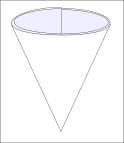
\includegraphics[width=0.5\linewidth]{Figures/rp1.png}
    \caption*{}
    \label{fig:my_label}
\end{figure}
\pagebreak
\section{Relative Space and Quantization}
\subsection{Classical Theory of Identical Particles II}
We noticed in the last section that given a configuration space $\mathcal{M} \equiv (\RR^n)^{\times N}/\sim$, we could rewrite the space in the center-of-mass coordinates to find that $\mathcal{M} = \RR^n \times r(N,n)$, where $r(N,n)$ looks locally like $\RR^{n(N-1)}$ but with a few nasty extra features. The difference between the two manifests in the global (topological/geometric) properties of the spaces. Particularly in the analysis of \textit{parallel transport} and \textit{tangent vectors}. Though we haven't talked in detail about what a tangent vector is, for now we can use our intuition about velocity vectors - it is a vector valued object defined at each point along some curve or surface, and in this particular case we require the vector to be in some sense 'tangent' to the surface. You will see these notions defined in more detail in courses on general relativity or differential geometry, and the geometry of configuration spaces is very closely related to what we call 'gauge theories', which you will see later on as well. If you would like the full picture, it would be beneficial to spend some time studying what is called the \textit{tangent bundle} of a manifold.

Let's now use our intuition about velocity to consider some configuration spaces. We say that a velocity vector $v$ is a 'tangent vector to the configuration space', meaning that there is some curve through $\mathcal{M}$ which has velocity $v$ at some point $x$. As an example, in $\RR^2$ a particle requires both position and velocity in order for you to fully specify its' state - we therefore say that the \textit{state} of the particle is the pair $(x,v)$. In a simple space such as $\RR^2$, comparing the velocities of particles is simple, but we often take for granted the process of adding vectors 'tip to tail'. This way of comparing velocities is where you take the velocities as vectors in $\RR^2$ and subtract them pointwise. This works in $\RR^n$ easily, but you have to be more careful when considering so-called 'tangent vectors', which exist in a more complicated space called the tangent space. The tangent space is defined separately at each point in the 'ambient space' (here being \textrm{M}). For $\RR^2$, this is simply $\RR^2$ everywhere. But for an arbitrary manifold $\mathcal{M}$, the tangent space may be different at each point. Therefore we would like a way to transport velocities between tangent spaces in a continuous/parallel way. This is called parallel transport.
\pagebreak

\begin{figure}[ht]
    \centering
    \includegraphics[width=\linewidth]{Figures/figure3.png}
    \caption*{}
    \label{fig:21}
\end{figure}
The above diagram demonstrates this notion of parallel transport in $\RR^2$. Luckily, in euclidean space it does not matter what path we transport $v_2$ along. But there is a simple example where parallel transport fails! Imagine a curve which goes from some point to the north pole, changes direction, comes back down to the original latitude, and goes back to its' origin. A diagram will help.
\begin{figure}[h]
    \centering
    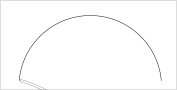
\includegraphics[width=\linewidth]{Figures/spheretransport.png}
    \caption*{}
    \label{fig:22}
\end{figure}

You will notice that if you draw vectors which \textit{stay tangent to the surface of the sphere}, then they change direction slightly as you move across the surface of the sphere. A vector (as shown in the diagram) which starts tangent to a line of latitude will eventually end up being perturbed by the motion.
\pagebreak
%22 minutes into lecture 2
\end{document}
